\chapter{Presentation of Results}
\section{Introduction}
The sections and subsections in this chapter describe the implementation, testing and results of the project. It starts by discussing how the web application to handle students' results was built. It then describes how The decentralised file storage element of the system was put up and how all these elements were integrated together.

\section{System Implementation}
This section and the subsections beneath it describe the Implementation and results of the project. Different elements of the system were built using different tools. The subsections below further describe how each element was built to get the complete system running from the web application that handles the students' results to the decentralised storage of transcripts and blockchain store for the hash values.

\subsection{Results System}
The results system is an element of the system where results are initially entered and processed before they are finally stored on a decentralised network. This system is built to be accessed by students, administrative assistants, the academic registrar and the system administrator. All these have different levels of priviledges when accessing the system for example, a student is only able to view his results and not edit them. The first attempt to build this system was done entirely on a blockchain network using smart contracts. 

\subsection{IPFS integration}
IPFS is a protocol that establishes the peer-to-peer network with resources addressed based on their content instead of the physical location. Our system uses this protocol with aim of guaranteeing users a decentralized and unalterable storage at a fraction of the price they  would have to give in transaction fees.\\
The PDF file generated by the Results system implementation above is the input of this next phase of imlementation.\\
We implement this protocol in such a way that the network is not going to store files once you add them. Adding files to IPFS does not upload them anywhere and only means that you add them to the local repository you host on your node. Therefore, what our system does is we create a hashed representation of the file and share this as a reference to the file.\\\\
XXXXXXXXXXXXXXXXXXXXXXXXXXXXXXXXXXXXXXXXXXXXXXXXXXXXXXXXXXXXXXXXXXXXXXXXXXXXXXXXXXXXXXXXXXXXXXXXXXXXXXXXXXX
\\\\
However, during the implementation of this project, we realized that connecting to the Ethereum blockchain is messy and complicated. We faced challenges which include:
\begin{enumerate}
\item The expense of storing data on the Ethereum blockchain
\item Complexity in configuring the Ethereum geth client and
\item Scalability of infrastructure would be tough
\end{enumerate}
\subsubsection{Infura}
In attempt to overcomethe challenges listed above, we used Infura. Infura is a set of tools used to create an application that connects to the Ethereum blockchain. It interacts with the Ethereum blockchain and runs nodes on behalf of our system.\\\\
Using Infura's API made our system fast, scalable and provides extra data storage. However, despite the fact that Infura offers to do that work for us, it brings with it the cost of increased centralization.
The output of this subsystem is a hashed  URL which is a reference to our PDF file.

\subsection{Ethereum blockchain}
As mentioned in the above section, using Infura and IPFS provides extra data storage for us. This is done is such a way that instead of storing the entire file on-chain, data can be stored separately i.e locally on a server from the results system in section 5.2.1, with just a hash stored on the blockchain.\\By storing the hash on the Ethereum blockchain,the system takes advantage of the blockchain principles of Immutability, Disintermediation and Transparency.
STILL WORK IN PROGRESS HERE
XXXXXXXXXXXXXXXXXXXXXXXXXXXXXXXXXXXXXXXXXXXXXXXXXXXXXXXXXXXXXXXXXXXXXXXXXXXXXXXXXXXXXXXXXXXXXXXXX
\begin{figure}[!h]
\center
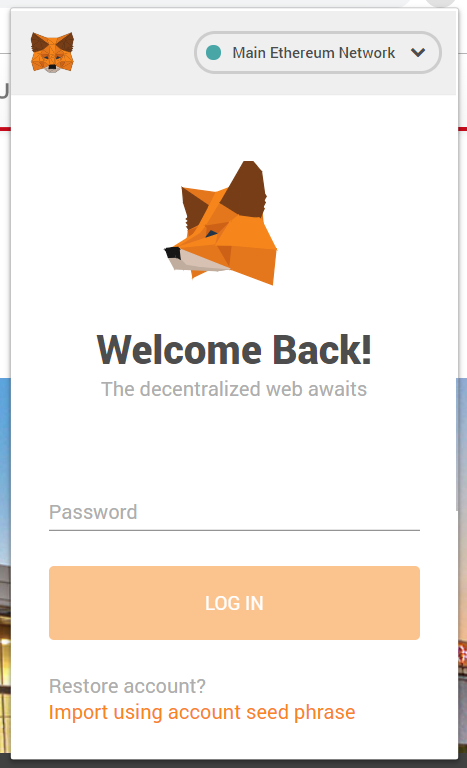
\includegraphics[scale=0.6]{images/metamasklogin.png}
\caption{Loging into the ethereum network}
\end{figure}

\subsubsection{Results}
\textbf{Viewing Results}\\~\\
This page can be accessed by a logged in student or an administrative assistant. The student can only view his/her results whereas the administrative assistant can view the results of various students.
\textbf{Manipulating results}\\~\\
In addtion to viewing results of various students, the adminsstrative assistant can also add/edit students’ results.
